%!TeX program = xelatex
\documentclass[12pt,a4paper,UTF8]{ctexart}

\usepackage[left=2.5cm,right=2.5cm,top=2.5cm,bottom=2.5cm]{geometry}
\usepackage{amsmath,amssymb}
\usepackage{booktabs}
\usepackage{graphicx}
\usepackage{float}
\usepackage{tabularx}
\usepackage{array}
\usepackage{xcolor}
\usepackage{listings}
\usepackage{hyperref}
\usepackage{fancyhdr}
\usepackage{longtable}
\usepackage{caption}
\usepackage{subcaption}

\graphicspath{{figures/}}
\hypersetup{colorlinks=true,linkcolor=black,urlcolor=blue,citecolor=blue}
\urlstyle{tt}
\setlength{\headheight}{15pt}
\setlength{\emergencystretch}{3em}
\pagestyle{fancy}
\fancyhead[L]{信息安全技术}
\fancyhead[C]{期末课程报告}
\fancyhead[R]{大语言模型文本水印}

\lstset{
    basicstyle=\ttfamily\small,
    breaklines=true,
    frame=single,
    columns=fullflexible,
    keepspaces=true
}

\newcommand{\method}{CA-KL}
\newcommand{\fullmethod}{CA-KL-CG}
\newcommand{\codepath}[1]{\textcolor{blue!45!black}{\nolinkurl{#1}}}

\begin{document}

\begin{titlepage}
    \centering
    \vspace*{1.2cm}
    
\includegraphics[width=0.48\textwidth]{sysu.jpg}
    \vspace{1.8cm}

    {\zihao{2}\heiti 信息安全技术课程期末报告\par}
    \vspace{1.1cm}
    {\zihao{3}\heiti 基于 KL 约束生成与匹配检测的大语言模型文本水印改进研究\par}
    \vspace{0.5cm}
    {\zihao{4} 基于 ICML 2023 论文 \textit{A Watermark for Large Language Models} 的复现与改进\par}

    \vfill
    \begin{tabular}{rl}
        学生姓名： & 施煌，祖裕柏，黄镇邦 \\
        学号： & 23336204，23344188，23342035 \\
        院系： & 计算机学院 \\
    \end{tabular}
    \vfill
    {\large 2026 年 7 月}
\end{titlepage}

\begin{abstract}
本报告围绕大语言模型生成文本的溯源问题展开，以 ICML 2023 论文 \textit{A Watermark for Large Language Models} 中的 KGW 文本水印为复现对象。原始 KGW 方法通过 seeded greenlist 在生成阶段对部分 token 施加固定 logits 偏置，并在检测阶段统计 green token 的异常比例。固定偏置方法具有实现简单、检测统计量清晰等优点，但也把所有生成位置视为同等可嵌入，难以区分高不确定位置和高置信位置的扰动代价。

围绕这一问题，本文实现并比较了两类自适应水印方法。第一类是基于熵的 Adaptive Delta，根据 next-token 分布熵调整每一步的偏置强度；第二类是本文重点采用的 \method{} Watermark，它在每一步通过 KL 散度预算约束加水印分布 $P'_t$ 与原始分布 $P_t$ 的距离，并在预算内选择最大可用偏置。在此基础上，\fullmethod{} 进一步引入 candidate-aware greenlist 与 confidence gate，使水印主要作用于候选空间内、模型分布更适合嵌入的位置。检测端实现了模型辅助的 entropy-weighted detector 和 windowed detector，用 weighted z-score、WinMax weighted z-score、AUC 与 TPR@FPR 评价自适应水印信号。

实验使用 \texttt{facebook/opt-2.7b} 与 C4/realnewslike 500 条样本。结果显示，\method{} 在普通 KGW 检测器下的检测成功率为 95.60\%，高于 \texttt{Fixed Delta 2.0} 的 92.80\% 和 Adaptive Delta 的 88.60\%。\fullmethod{} 在 gate 0.10/0.95 下的普通 KGW 检测率为 88.80\%，PPL 为 5.6073；在 matched weighted/WinMax 检测器下，weighted z-score 为 9.1174，AUC 为 0.9992，TPR@1\%FPR 为 99.60\%。实验表明，KL 预算能够为水印强度提供可解释约束，而模型辅助加权检测能够更充分地利用自适应生成过程中留下的水印证据。

\noindent\textbf{关键词：}大语言模型；文本水印；信息安全；KL 散度；加权检测；内容溯源
\end{abstract}

\clearpage
\pagenumbering{Roman}
\tableofcontents
\clearpage
\pagenumbering{arabic}

\section{引言}

大语言模型在内容生成、问答辅助、教育支持、编程协作等场景中已经表现出很强的实用价值，但与此同时，模型输出内容的可追踪性与可验证性问题也逐渐成为信息安全领域的重要研究方向。一方面，大模型生成文本在形式上越来越接近人工撰写内容，如果缺少额外标记，平台、教师、企业和监管者很难快速判断某段文本是否由模型生成；另一方面，生成式模型被广泛接入搜索、写作和社交平台之后，伪造信息、自动批量灌水、学术不端和内容归属不清等问题也更加突出。在这样的背景下，文本水印技术成为连接生成模型与内容治理的重要安全机制。与传统密码学中的加密或签名不同，文本水印不要求直接暴露密钥，也不要求改变文本的外部显示格式，而是通过对生成过程施加概率偏置，使得文本在统计意义上带有可检测的“生成痕迹”。因此，围绕文本水印开展复现和改进，不仅契合《信息安全技术》课程中关于数字水印的主题，也具有很强的现实应用价值。

本文复现的原始论文是 Kirchenbauer 等人在 ICML 2023 发表的 \textit{A Watermark for Large Language Models}~\cite{kirchenbauer2023watermark}。该论文提出的 KGW 方法思路清楚、代码开源，适合作为课程大作业的基础。它在每一步生成前，根据已有上下文用伪随机方式把词表划分为 greenlist 和 redlist，然后给 greenlist 中的 token logits 加上固定偏置 \texttt{delta}。检测时使用同样的密钥和上下文重建 greenlist，再统计文本中 green token 的数量是否异常偏高，从而判断文本是否可能由带水印模型生成。

方法设计还参考了水印可靠性和自适应水印方向的后续工作。可靠性研究强调，水印检测不仅需要固定阈值，还应关注误报率、文本长度、攻击和统计校准等因素~\cite{kirchenbauer2024reliability}；自适应水印研究则指出，不同生成位置的可嵌入性存在差异，熵和模型置信度可以作为调节水印强度的重要信号~\cite{liu2024adaptive}。这两点共同引出本文的设计思路：生成端用 KL 预算约束扰动，检测端用加权和校准指标评价水印证据。

固定 \texttt{delta} 方法具有清晰的单调关系：偏置越大，green token 越多，检测越容易。然而不同 \texttt{delta} 的对比结果表明，强水印虽然能提高 z-score，也会更明显地干预模型原本的选择，使文本多样性下降、重复率上升。因此，改进目标不应只追求检测率，还应考虑如何在控制原始生成分布扰动的同时留下稳定的水印证据。

因此，本报告的改进目标是构建一种可解释的质量--检测折中机制。本文采用 KL 散度作为每一步分布扰动的预算，并配合加权检测器重新评估水印信号。水印强度不再被视为孤立超参数，而是与当前位置的模型分布、可嵌入性以及检测统计量共同设计。

\section{原论文方法阅读与复现}

\subsection{KGW 文本水印的基本机制}

KGW 方法的核心是 seeded greenlist。设词表大小为 $|\mathcal{V}|$，水印参数 $\gamma$ 控制 greenlist 占词表的比例。对于当前前缀 $x_{<t}$，算法用密钥和前缀生成伪随机种子，再由该种子把词表划分为 greenlist $G_t$ 和 redlist $R_t$。如果模型原始输出 logits 为 $l_t(v)$，水印生成器会对 $v\in G_t$ 的 token 加上固定偏置：
\[
l'_t(v)=
\begin{cases}
l_t(v)+\delta, & v\in G_t,\\
l_t(v), & v\notin G_t.
\end{cases}
\]
随后模型根据修改后的分布进行采样。这样生成出的文本不会在表面出现特殊符号，但 green token 的出现比例会高于自然文本。

检测端使用同样的种子规则逐 token 重建 greenlist，并统计生成文本中落入 greenlist 的 token 个数。假设无水印文本中每个 token 落入 greenlist 的概率约为 $\gamma$，长度为 $T$ 的文本中 green token 的期望数量为 $\gamma T$，方差为 $T\gamma(1-\gamma)$。因此原论文使用 z-score 衡量偏离程度：
\[
z=\frac{|s|_G-\gamma T}{\sqrt{T\gamma(1-\gamma)}}.
\]
其中 $|s|_G$ 是观测到的 green token 数量。z-score 越高，说明文本中 green token 多得越不正常，也就越支持该文本带有水印。论文同时给出 $p$-value 和阈值判断，因此它本质上不是训练一个二分类器，而是在生成过程里嵌入一种可重复验证的统计偏差。

从代码结构上看，官方实现主要由两个类支撑。生成阶段的 \texttt{WatermarkLogitsProcessor} 继承 Hugging Face 的 \texttt{LogitsProcessor}，在每一步生成前根据当前 prefix 计算 greenlist，并给 greenlist token 加上固定 \texttt{delta}。检测阶段的 \texttt{WatermarkDetector} 按照同样的 seeding 规则重建 greenlist，输出 \texttt{num\_green\_tokens}、\texttt{green\_fraction}、\texttt{z\_score}、\texttt{p\_value} 和最终 \texttt{prediction}。本文后续方法保留这一生成--检测密钥一致性，只改变水印强度控制和检测统计量。

\subsection{官方仓库与复现环境}

复现工作从官方仓库 \codepath{jwkirchenbauer/lm-watermarking} 开始。这个仓库包含 \codepath{demo_watermark.py}、\codepath{watermark_processor.py}、\codepath{extended_watermark_processor.py}、\codepath{normalizers.py} 和 \codepath{alternative_prf_schemes.py} 等核心文件，其中最关键的是 \codepath{watermark_processor.py}，它实现了基础 KGW 水印生成器和检测器。图~\ref{fig:official-repo} 展示了复现所使用的官方仓库页面，后续课程代码也是在该仓库结构上整理出来的。

\begin{figure}[H]
    \centering
    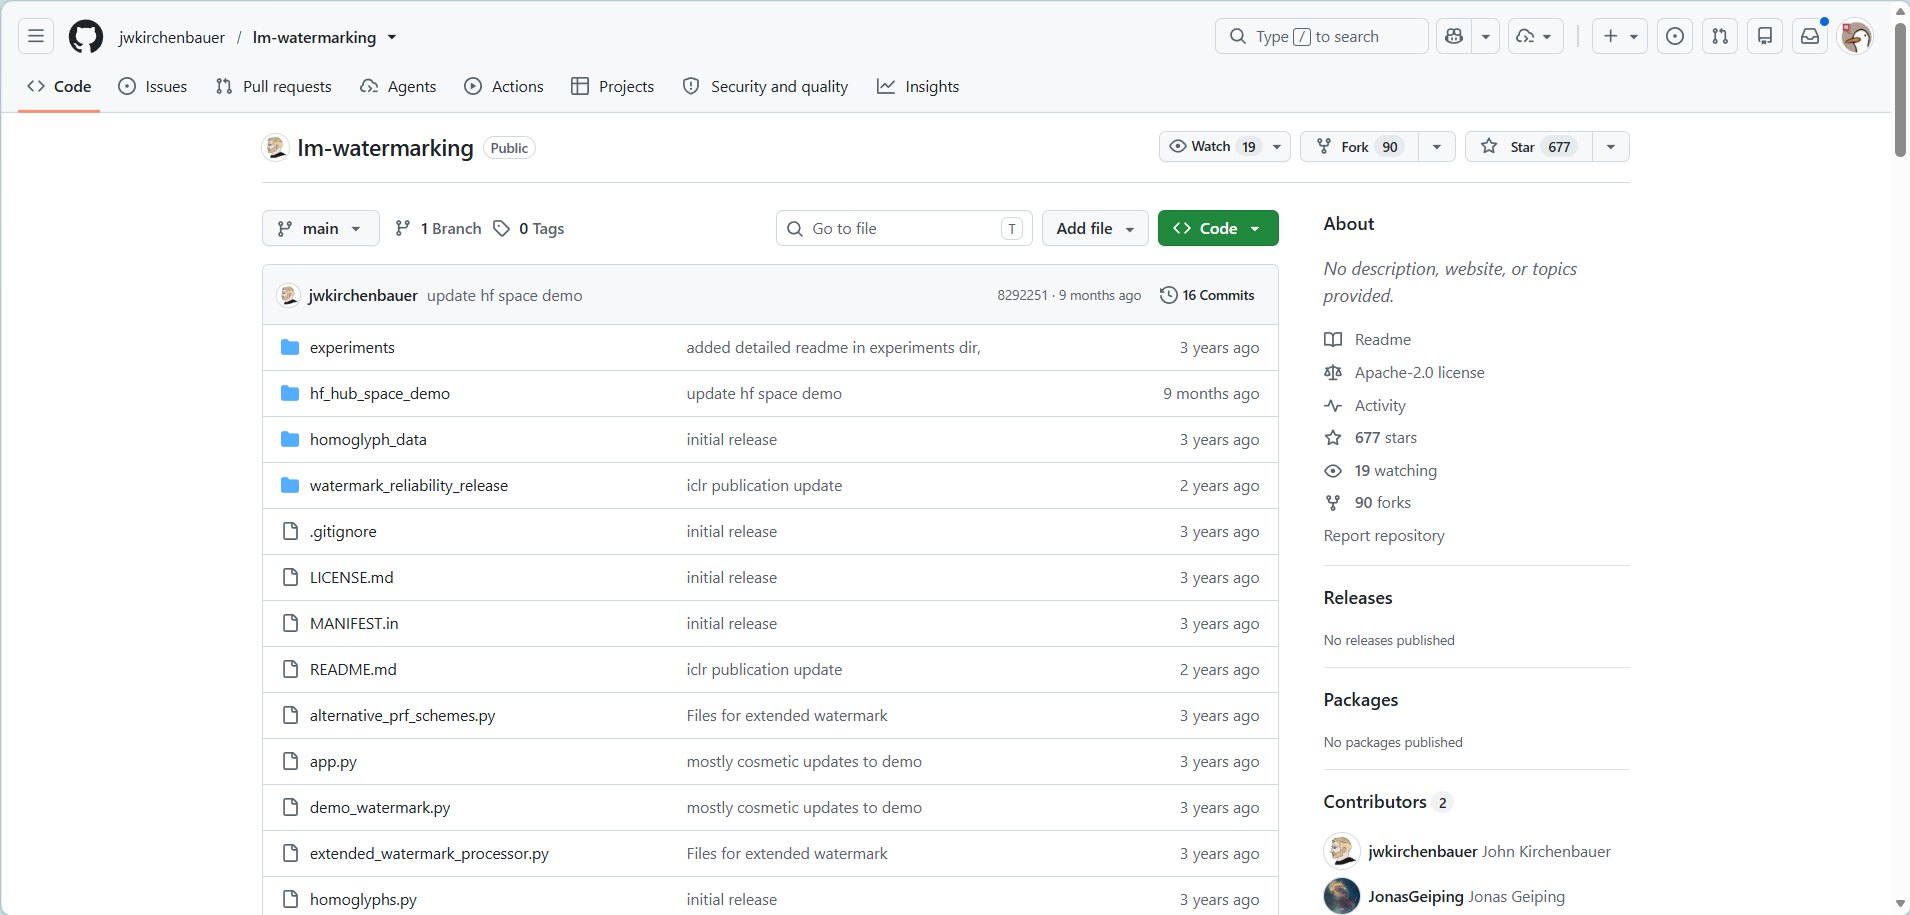
\includegraphics[width=0.92\textwidth]{official_repo.png}
    \caption{官方 lm-watermarking 仓库页面}
    \label{fig:official-repo}
\end{figure}

复现与后续实验基于 Anaconda 环境完成。正式实验环境使用 \texttt{pytorch} conda 环境，核心依赖包括 PyTorch、Transformers、datasets、scipy、pandas 和 matplotlib。模型方面，复现阶段先使用 \texttt{sshleifer/tiny-gpt2} 跑通官方 Demo，因为它下载快、显存压力小，适合排查环境和接口问题；确认生成、检测、CSV 输出和绘图流程没有问题后，再下载并使用 \texttt{facebook/opt-2.7b} 作为正式实验模型。

为保持复现代码和课程改进代码的边界，新增内容集中放在 \codepath{course_project/} 目录下。其中 \codepath{processors/} 保存改进后的 logits processor 和 detector，\codepath{scripts/} 保存批量实验、prompt 准备和结果分析脚本，\codepath{outputs/} 保存 CSV、Markdown 摘要和图表。该组织方式便于在不改动原始 \codepath{watermark_processor.py} 的前提下，比较固定 \texttt{delta}、Adaptive Delta、\method{} 和 \fullmethod{}。

\subsection{原始复现步骤}

官方复现按照“仓库准备、依赖安装、模型下载、Demo 启动、结果验证”的顺序完成。复现阶段先用最小模型跑通完整链路，以便提前暴露 Gradio、Transformers 和本地模型路径的问题。核心命令如下：

\begin{lstlisting}[language=bash]
git clone https://github.com/jwkirchenbauer/lm-watermarking.git
cd lm-watermarking
conda create -n inform python=3.10 -y
conda activate inform
pip install -r requirements.txt
\end{lstlisting}

模型准备完成后，使用本地 tiny-gpt2 启动官方 Gradio Demo：

\begin{lstlisting}[language=bash]
python demo_watermark.py \
  --model_name_or_path ./models/tiny-gpt2 \
  --use_gpu True \
  --run_gradio True \
  --max_new_tokens 100
\end{lstlisting}

复现过程中遇到的一个实际问题是 Gradio 版本兼容。官方旧代码中使用的 \texttt{demo.queue(concurrency\_count=3)} 在新版 Gradio 中已经不再兼容，启动时会报参数错误。将其改为 \texttt{demo.queue(default\_concurrency\_limit=3)} 后，前端页面可以正常打开。该修复本身不改变水印算法，只是让官方交互式 Demo 能在当前环境下运行。图~\ref{fig:official-demo-start} 展示了官方 Demo 正常启动后的界面。

\begin{figure}[H]
    \centering
    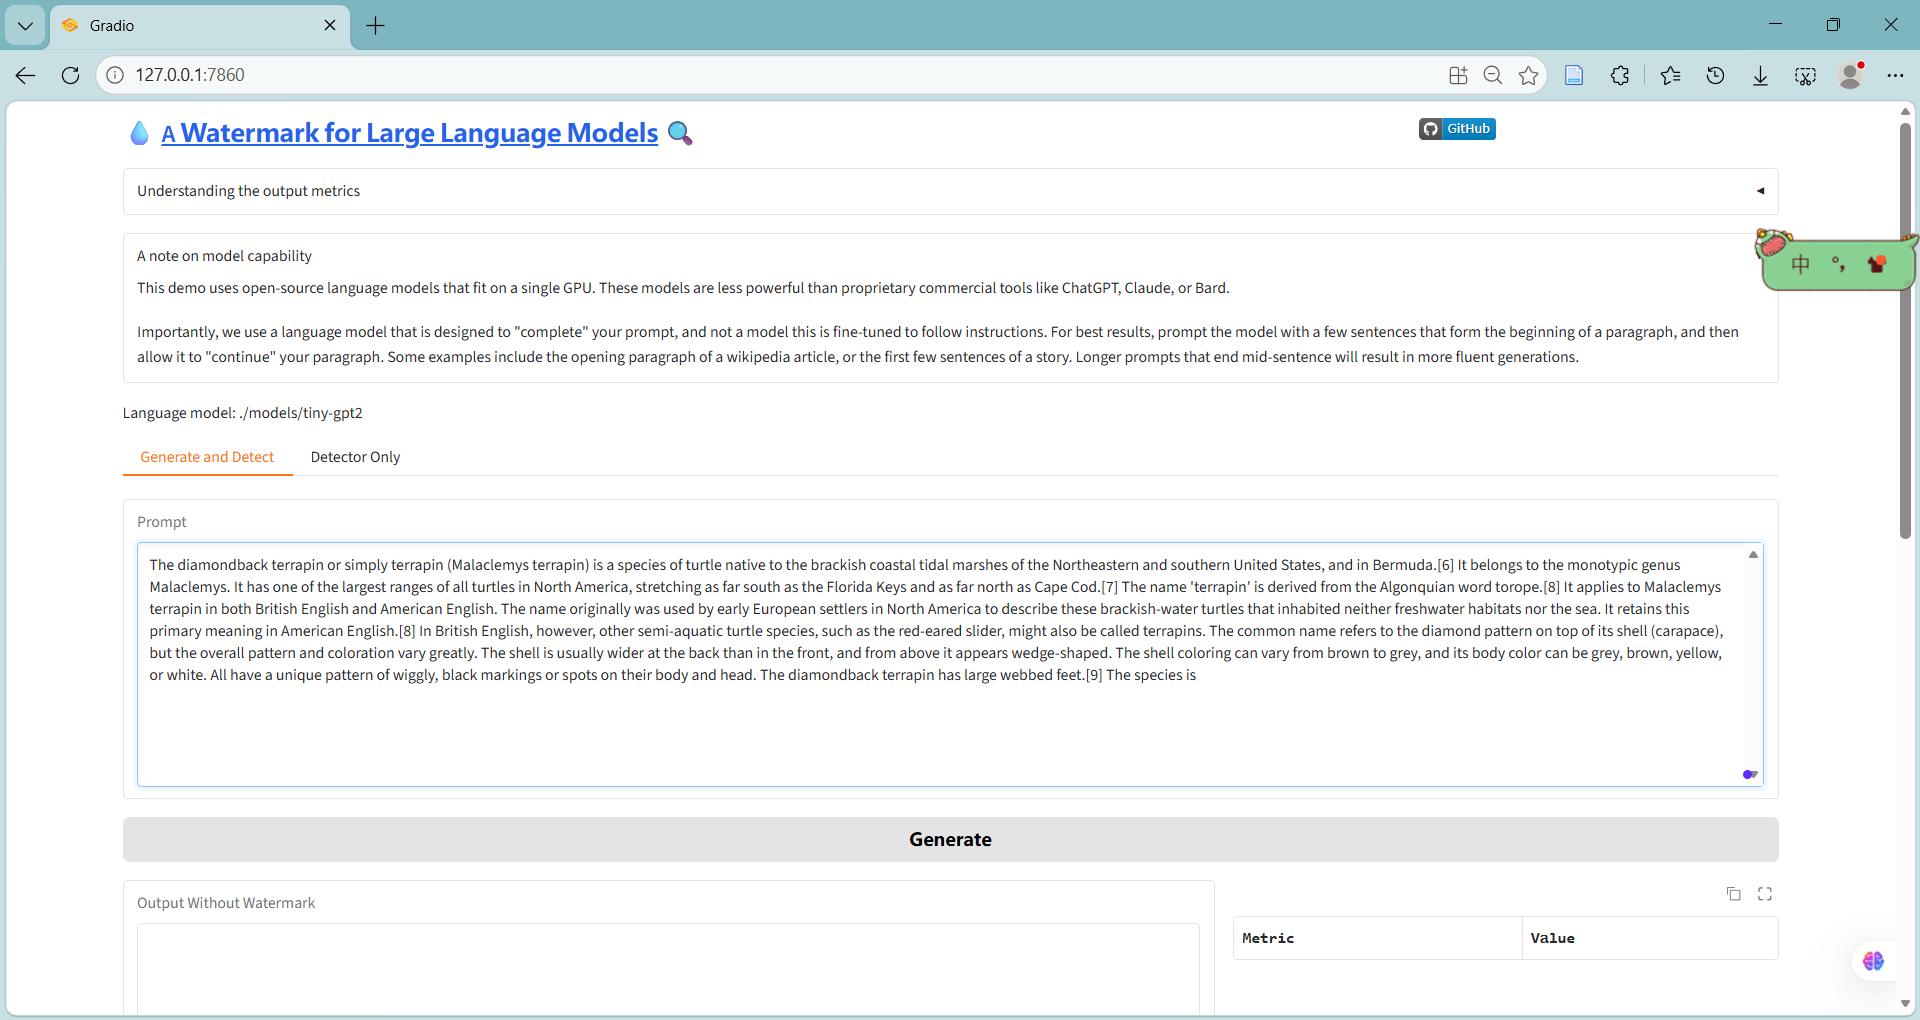
\includegraphics[width=0.92\textwidth]{official_demo_start.png}
    \caption{官方 Gradio Demo 启动界面}
    \label{fig:official-demo-start}
\end{figure}

\subsection{复现结果与验证}

官方 Demo 的验证方式很直接：输入同一个 prompt，系统同时生成无水印文本和带水印文本，并在右侧输出各自的检测统计量。一次典型复现结果如图~\ref{fig:official-demo-detection} 所示，无水印文本统计到 $T=99$ 个 token，其中 green token 数量为 22，\texttt{green\_fraction} 为 22.2\%，\texttt{z-score=-0.638}，检测结果为 \texttt{Human/Unwatermarked}；带水印文本统计到 $T=98$ 个 token，其中 green token 数量为 69，\texttt{green\_fraction} 为 70.4\%，\texttt{z-score=10.4}，检测结果为 \texttt{Watermarked}，置信度接近 100\%。

\begin{figure}[H]
    \centering
    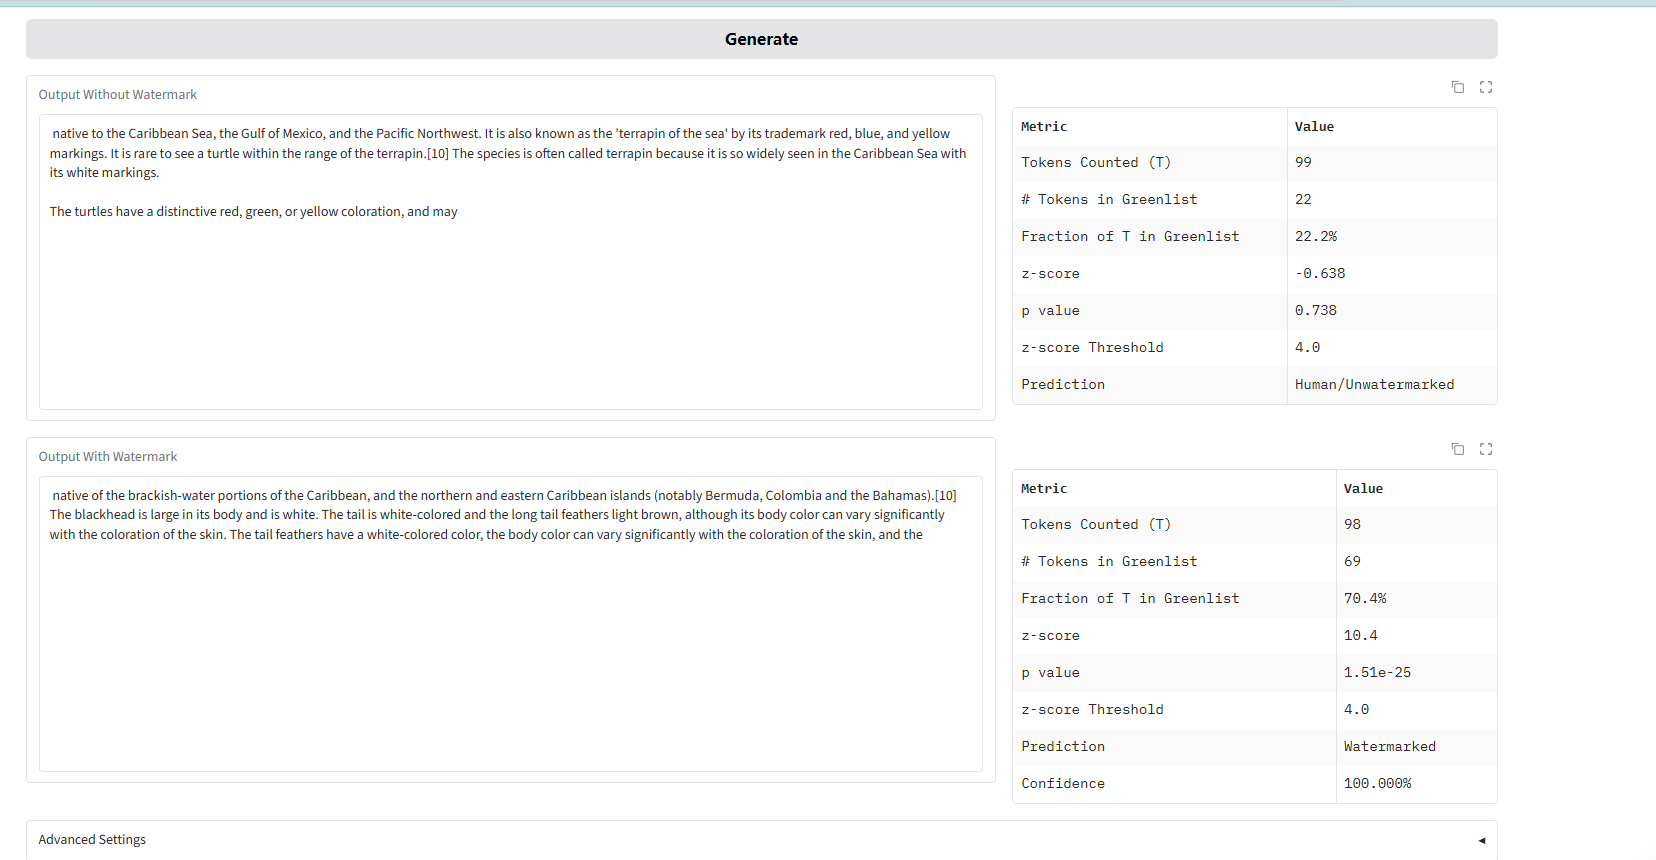
\includegraphics[width=0.92\textwidth]{official_demo_detection.png}
    \caption{官方 Demo 中无水印文本与带水印文本的检测结果}
    \label{fig:official-demo-detection}
\end{figure}

该结果展示了原论文方法的基本特征：水印并不是在文本表面添加某个特殊符号，而是在生成概率里持续施加很小的统计倾向；单个 token 看起来仍然自然，但几十个 token 累积后，green token 占比会显著偏离自然文本。也正因为这一点，z-score 成为后续实验最重要的检测指标之一。

\subsection{复现中观察到的问题}

完成官方 Demo 复现后，批量脚本进一步比较了不同固定 \texttt{delta} 的效果。\texttt{delta} 越大，green fraction 和 z-score 越高，检测成功率也越高；同时，强水印也会带来更明显的分布扰动。以 500 条 OPT-2.7B fp32 实验为例，\texttt{Fixed Delta 3.0} 的普通 KGW 检测成功率达到 98.40\%，平均 z-score 达到 10.0975，但 continuation PPL 升到 7.0199，明显高于无水印文本的 4.1244。\texttt{Fixed Delta 2.0} 的检测成功率为 92.80\%，PPL 为 5.4301；\texttt{Fixed Delta 1.7} 检测成功率为 82.00\%，PPL 为 4.9519。固定 \texttt{delta} 曲线提供了重要参照：强水印更容易检测，但流畅度和分布保持会付出代价。

固定 \texttt{delta} 的主要限制不在于检测能力不足，而在于它把所有生成位置当成一样处理。有些位置模型本来就非常确定，例如固定搭配、常见虚词或标点附近，强行推动 green token 更容易伤害自然性；有些位置模型有多个合理候选，此时嵌入水印的代价更低。原始方法没有区分这种差异，这构成了本文自适应水印方法的切入点。

\section{自适应水印方法设计}

\subsection{基于熵的 Adaptive Delta}

Adaptive Delta 方法利用 next-token 分布熵刻画当前位置的生成不确定性。设当前分布的归一化熵为 $H_{\text{norm}}$，水印偏置由如下经验函数给出：
\[
\delta_t=\delta_{\min}+(\delta_{\max}-\delta_{\min})\cdot f(H_{\text{norm}}).
\]
该方法比固定 \texttt{delta} 更灵活，也具有直观解释：高熵位置有更多合理候选，适合使用更强水印；低熵位置更确定，适合使用较小偏置。

Adaptive Delta 的不足在于，熵到 \texttt{delta} 的映射仍然依赖经验参数，难以直接说明某个熵值对应某个具体偏置的分布意义。此外，若检测端仍然使用原始 KGW detector，则检测统计量没有显式利用生成端的可嵌入性差异。本文将 Adaptive Delta 作为重要对照方法，并进一步引入 KL 约束来重新定义每一步允许施加的水印强度。

\subsection{使用 KL 约束重新定义水印强度}

本文将水印强度控制改写为一个受约束的选择问题：每一步不直接指定 \texttt{delta}，而是在可接受的分布扰动预算内，选择尽可能大的水印偏置。设原始模型分布为 $P_t$，加水印后的分布为 $P'_t$，约束定义为：
\[
D_{\mathrm{KL}}(P'_t\|P_t)\leq \varepsilon.
\]
该约束的含义是：水印可以改变模型分布，但这种改变不能超过预设预算 $\varepsilon$。在实现中，首先计算当前 greenlist 在原始分布下的概率质量 $p_G$，再对 $\delta_t$ 做二分搜索。对于给定 $\delta$，归一化因子为：
\[
Z=1+(\exp(\delta)-1)p_G,
\]
加水印后 greenlist 的总概率质量为：
\[
q_G=\frac{\exp(\delta)p_G}{Z},
\]
对应的 KL 散度可以写成：
\[
D_{\mathrm{KL}}(P'_t\|P_t)=\delta q_G-\log Z.
\]
本文选择满足 KL 预算的最大 $\delta_t$。这样一来，水印强度不再由熵的经验映射给出，而是由当前分布和 KL 预算共同决定。小规模网格实验显示，$\varepsilon=0.02$ 时平均 \texttt{delta} 过低，检测信号不足；$\varepsilon=0.50$ 能使水印信号进入稳定可检出区间。在 500 条 OPT-2.7B fp32 实验中，\method{} 的平均自适应 \texttt{delta} 为 2.5108，既能形成明显水印痕迹，也保留了分布约束的解释。

\subsection{加权检测器的作用}

在生成端引入自适应强度后，检测端也需要相应调整。原始 z-score 把每个 token 位置等权看待，但在自适应水印中，每个位置的可嵌入性并不一样。为使检测器与生成机制更一致，本文实现了模型辅助的 entropy-weighted detector。检测时，系统用同一个基础模型重新计算每个 prefix 的 logits，得到当前位置的熵、候选 greenlist 及其概率质量，并对高熵位置赋予更高权重。

本文将生成端机制和检测端机制分开定义。\method{}、candidate-aware greenlist 和 confidence gate 属于生成端机制，决定文本如何被加水印；weighted detector 和 WinMax detector 属于检测端机制，决定同一段文本如何被评分。因此，``\method{} + Weighted Detector'' 表示对 \method{} 生成文本使用模型辅助检测器评分；完整方案可表述为 ``\fullmethod{} 生成 + weighted/WinMax 检测''。

加权检测的统计量为：
\[
Z_w=\frac{\sum_i w_i(G_i-p_i)}
{\sqrt{\sum_i w_i^2p_i(1-p_i)}}.
\]
其中 $G_i$ 表示第 $i$ 个生成 token 是否落入 greenlist，$p_i$ 是无水印条件下落入该 greenlist 的概率质量，$w_i$ 是由当前 prefix 分布计算出的权重。由于 $w_i$ 只依赖当前 token 之前的 prefix，不依赖当前 token 是否命中 greenlist，这个统计量在无水印文本下仍然有合理的零均值解释。

此外，本文还实现了 windowed detector，即在多个窗口长度上计算局部加权 z-score，并取最大值。这个设计主要面向 copy-paste 混入场景：如果一段带水印文本被插入到大量无水印文本中，全局统计量会被稀释，而窗口检测可以更容易发现局部水印片段。

\section{实现细节}

代码实现主要增加了三个部分。第一，\codepath{course_project/processors/cakl_watermark_processor.py} 中实现了 CA-KL 生成器，负责 KL-constrained adaptive delta、confidence gate 和 candidate-aware greenlist。第二，同一文件中实现了模型辅助检测器，负责 weighted z-score 和 WinMax weighted z-score。第三，\codepath{course_project/scripts/run_experiments.py} 被扩展为批量实验入口，用于比较 \texttt{No Watermark}、多个固定 \texttt{delta}、Adaptive Delta、\method{} 生成、\method{} + Candidate Greenlist 生成，以及 \fullmethod{} 生成在普通 KGW 检测器和加权检测器下的表现。

实现中保持三个原则。首先，模型不做 fine-tuning，所有水印都在 inference-time 修改 logits，以保持方法与原论文设定一致。其次，保留普通 KGW 检测器，用于和固定 \texttt{delta} baseline 做同口径比较；模型辅助加权检测器则作为匹配 \method{} 和 \fullmethod{} 的增强检测口径。最后，结果分析脚本同时输出平均 z-score、普通检测成功率、AUC、TPR@1\%FPR、TPR@5\%FPR、平均 KL 和平均自适应 \texttt{delta} 等指标。

核心实验脚本如下，分别对应完整 baseline 对比、confidence gate 网格、选定 gate 下的 \method{} 系列实验，以及 \texttt{Fixed Delta 1.7} 对照实验：
\begin{lstlisting}[language=bash]
bash course_project/scripts/run_opt27b_full_500_fp32.sh
bash course_project/scripts/run_opt27b_gate_grid_fp32.sh
bash course_project/scripts/run_opt27b_full_500_fp32_gate010_095.sh
bash course_project/scripts/run_opt27b_fixed17_500_fp32.sh
\end{lstlisting}

\section{实验设置}

正式实验使用 \texttt{facebook/opt-2.7b}，该模型来自 OPT 开放预训练模型系列~\cite{zhang2022opt}。数据来自 C4/realnewslike，C4 本身是大规模清洗网页文本数据集~\cite{raffel2020exploring}。实验使用保存好的 500 条 prompt，每条最多生成 100 个 token；模型以 fp32 加载，并在共享服务器上通过 \texttt{CUDA\_VISIBLE\_DEVICES} 指定单张 GPU 运行。

\begin{table}[H]
    \centering
    \caption{正式实验设置}
    \label{tab:setup}
    \begin{tabularx}{0.92\textwidth}{p{0.30\textwidth}X}
        \toprule
        项目 & 设置 \\
        \midrule
        基础模型 & \texttt{facebook/opt-2.7b} \\
        数据集 & \texttt{C4/realnewslike}，保存为 \texttt{prompts\_c4\_realnewslike\_500.txt} \\
        正式评估样本数 & 500 条 prompt \\
        每条最大生成长度 & 100 tokens \\
        采样方式 & multinomial sampling，temperature = 0.7 \\
        水印比例参数 & $\gamma=0.25$ \\
        原始检测阈值 & z-score threshold = 4.0 \\
        \method{} 参数 & $\varepsilon=0.50$，\texttt{delta\_max=3.0} \\
        Confidence Gate & $H_{\text{norm}}\geq 0.10$，$p_{\text{top1}}\leq 0.95$ \\
        Candidate Greenlist & \texttt{top\_p=0.95} \\
        硬件 & 共享服务器单卡 GPU，fp32 加载 \\
        \bottomrule
    \end{tabularx}
\end{table}

评价指标分为三类。第一类是原始 KGW 检测指标，包括 green fraction、普通 z-score 和普通 detection success rate；其中 success rate 指文本在原始 KGW 检测器下被判定为 \texttt{Watermarked} 的比例。第二类是文本质量指标，包括 continuation PPL、Distinct-1、Distinct-2 和 Repetition Rate；PPL 越低说明生成文本越接近原模型分布，Distinct 越高通常说明文本越不重复，Repetition Rate 越低说明词汇重复越少。第三类是匹配自适应生成机制的增强检测指标，包括 Weighted z-score、WinMax Weighted z-score、AUC 和 TPR@FPR。这三类指标回答的问题不同：普通 KGW 指标衡量与原论文检测器的兼容性，加权检测指标衡量模型辅助检测是否能捕捉自适应水印信号，质量指标衡量生成扰动带来的副作用。

\section{实验结果}

\subsection{主结果对比}

\begin{table}[H]
    \centering
    \caption{OPT-2.7B + C4/realnewslike 500 条样本的普通 KGW 检测与 PPL 结果}
    \label{tab:main-results}
    \scriptsize
    \setlength{\tabcolsep}{2.5pt}
    \begin{tabularx}{\textwidth}{p{0.30\textwidth}rrrrrr}
        \toprule
        生成方法 & KGW z & KGW 检出率 & Corpus PPL & 平均 $\delta$ & Distinct-1 & 重复率 \\
        \midrule
        No Watermark & -0.3780 & 0.20\% & \textbf{4.1244} & -- & 0.6998 & 0.3002 \\
        Fixed Delta 1.0 & 2.9412 & 25.40\% & 4.4996 & 1.0000 & 0.7031 & 0.2969 \\
        Fixed Delta 1.7 & 5.5349 & 82.00\% & 4.9519 & 1.7000 & 0.6981 & 0.3019 \\
        Fixed Delta 1.864 & 6.3353 & 89.60\% & 5.2054 & 1.8640 & 0.6967 & 0.3033 \\
        Fixed Delta 2.0 & 6.8200 & 92.80\% & 5.4301 & 2.0000 & 0.6935 & 0.3065 \\
        Fixed Delta 3.0 & \textbf{10.0975} & \textbf{98.40\%} & 7.0199 & 3.0000 & 0.6958 & 0.3042 \\
        Adaptive Delta & 6.2743 & 88.60\% & 5.1528 & -- & 0.7037 & 0.2963 \\
        \method{} & 7.5682 & 95.60\% & 5.8167 & 2.5108 & 0.7022 & 0.2978 \\
        CA-KL + Candidate Greenlist & 6.8102 & 92.40\% & 6.0565 & 2.4861 & \textbf{0.7086} & \textbf{0.2914} \\
        \fullmethod{}，gate 0.10/0.95 & 6.3873 & 88.80\% & 5.6073 & 1.6893 & 0.7057 & 0.2943 \\
        \bottomrule
    \end{tabularx}
\end{table}

表 \ref{tab:main-results} 采用普通 KGW 检测器，即每个 token 位置等权、统计 green token 偏离程度。\method{} 的普通检测成功率为 95.60\%，高于 \texttt{Fixed Delta 2.0} 的 92.80\% 和 Adaptive Delta 的 88.60\%；平均 z-score 也更高。这说明 KL 预算约束能够在不手动指定固定 \texttt{delta} 的情况下形成稳定的统计偏差。

PPL 结果体现了检测强度与分布扰动之间的权衡。\texttt{Fixed Delta 3.0} 的 KGW 检测最强，PPL 为 7.0199；\texttt{Fixed Delta 2.0} 的 PPL 为 5.4301，检测率为 92.80\%；\method{} 的检测率进一步提高到 95.60\%，PPL 为 5.8167。由此可见，\method{} 的优势主要体现在 KL 预算约束下的动态强度控制和更高检测信号。

\fullmethod{} 使用 gate 0.10/0.95 后，平均 \texttt{delta} 为 1.6893，接近补充实验中的 \texttt{Fixed Delta 1.7}。在相近平均强度下，\fullmethod{} 的普通 KGW 检出率为 88.80\%，高于 \texttt{Fixed Delta 1.7} 的 82.00\%；PPL 为 5.6073。该结果说明，candidate-aware greenlist 和 confidence gate 能在较低平均偏置下保留可检测信号，并为后续模型辅助检测提供更集中的统计证据。

\begin{figure}[H]
    \centering
    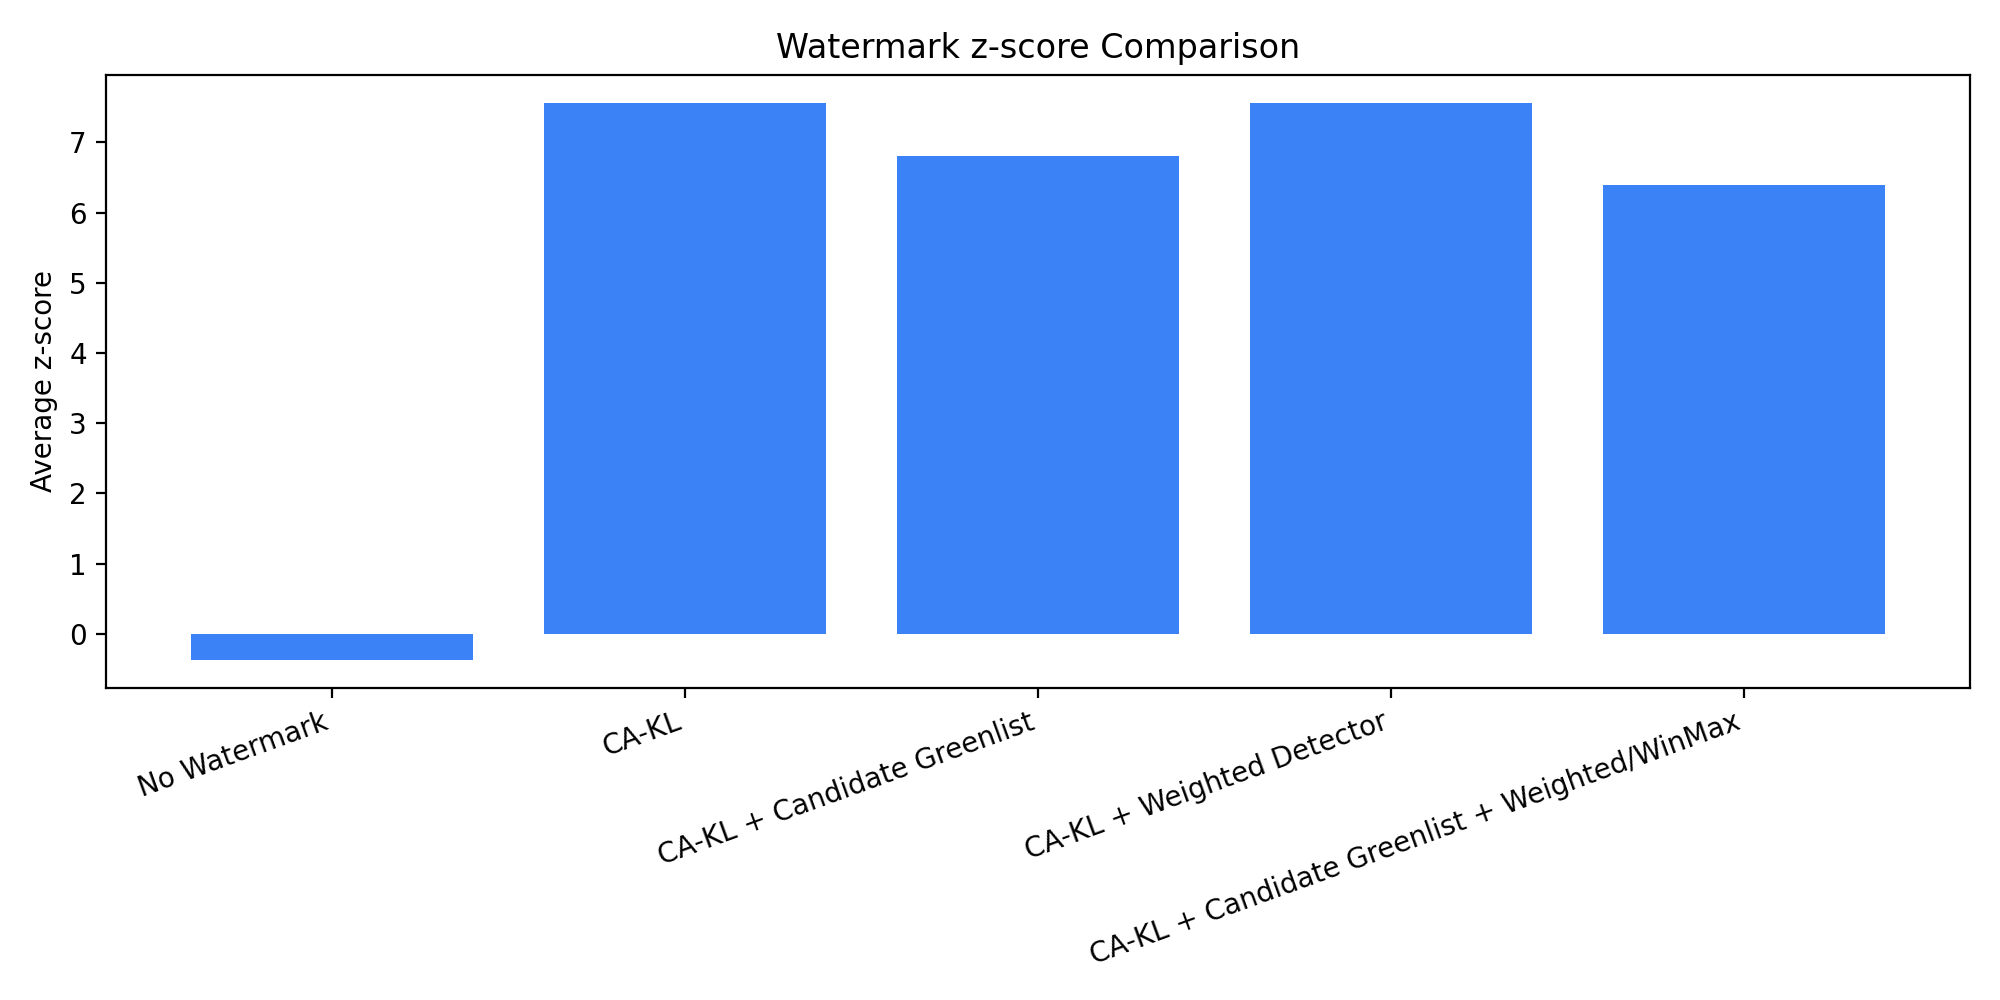
\includegraphics[width=0.86\textwidth]{cakl_zscore.png}
    \caption{选定 gate 0.10/0.95 下 CA-KL 系列的平均 z-score 对比}
    \label{fig:zscore}
\end{figure}

\begin{figure}[H]
    \centering
    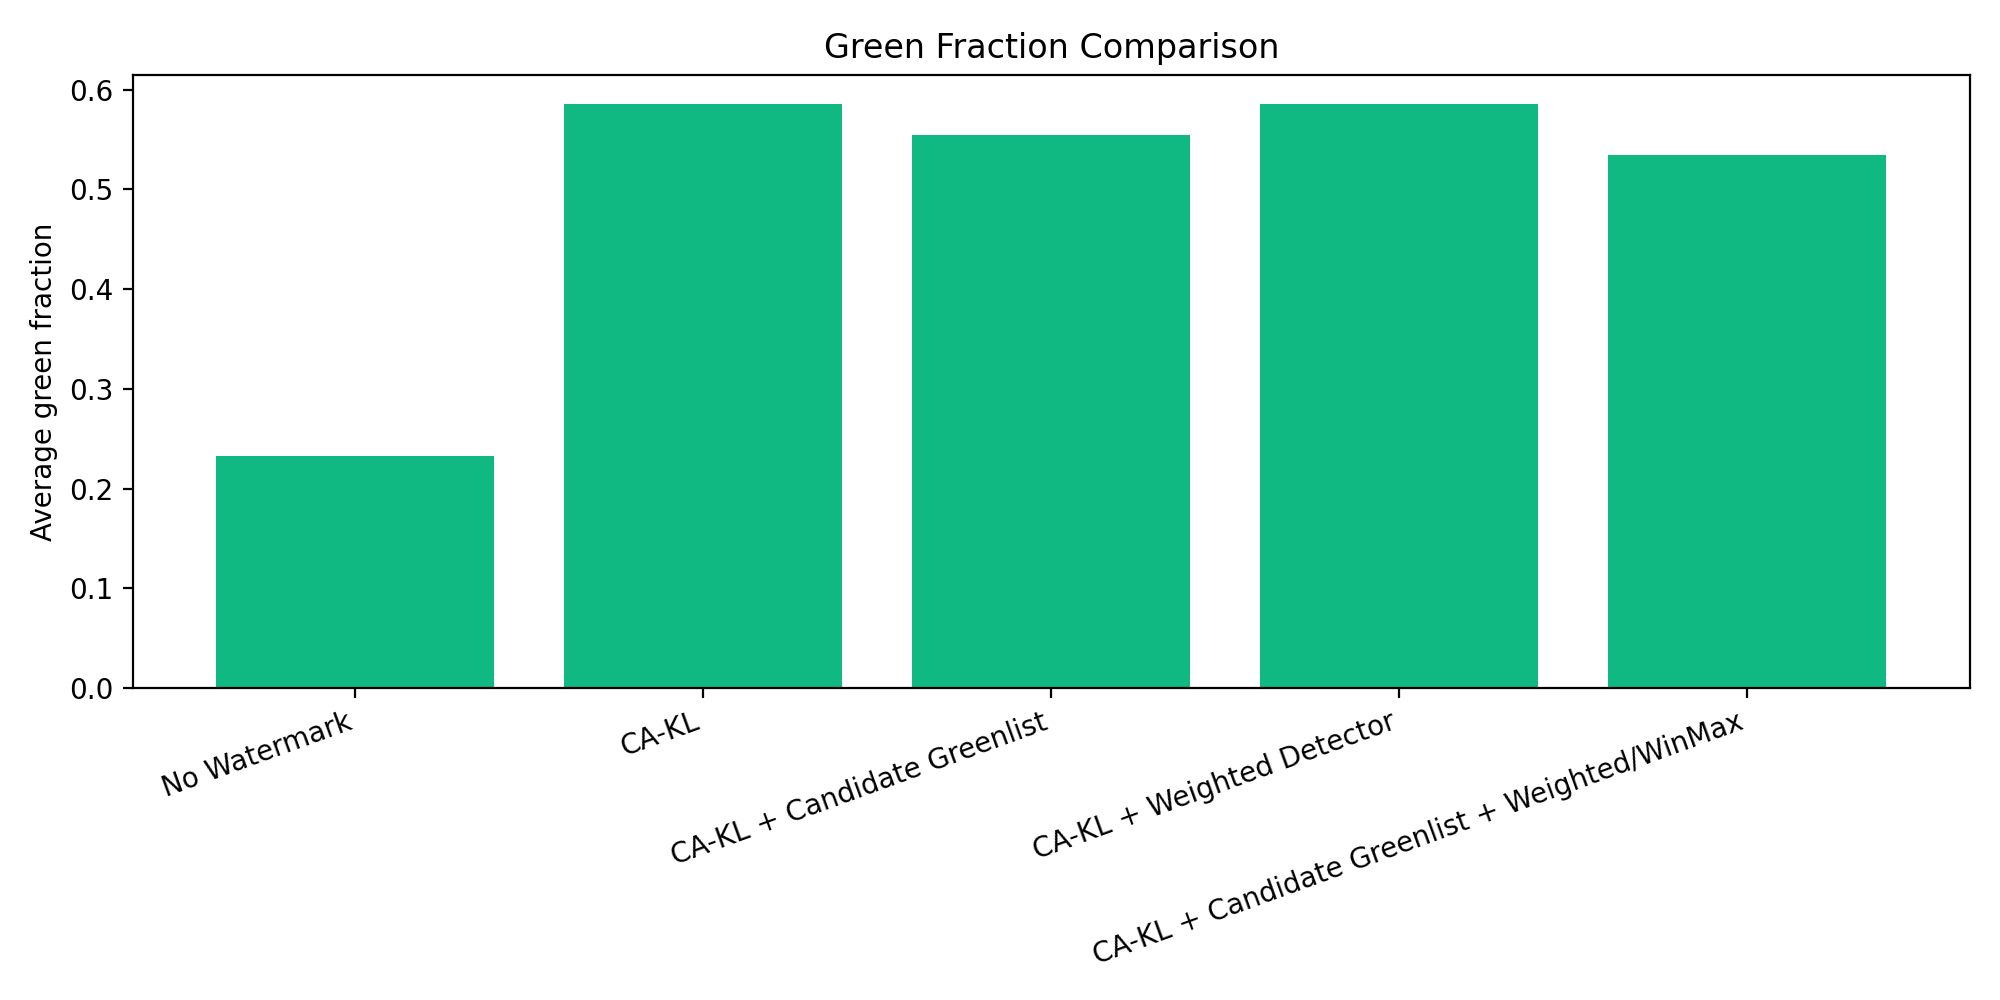
\includegraphics[width=0.86\textwidth]{cakl_green.png}
    \caption{选定 gate 0.10/0.95 下 CA-KL 系列的 green fraction 对比}
    \label{fig:green}
\end{figure}

\subsection{Confidence Gate 参数分析}

Confidence gate 控制 \fullmethod{} 的实际嵌入位置：只有当当前位置满足熵下界且 top-1 概率不超过给定阈值时，生成器才施加水印偏置。为了分析 gate 对水印强度的影响，实验比较了五组 $(H_{\text{norm}},p_{\text{top1}})$ 参数。结果见表 \ref{tab:gate-grid}。

\begin{table}[H]
    \centering
    \caption{50 条样本上 \fullmethod{} 的 confidence gate 网格结果}
    \label{tab:gate-grid}
    \scriptsize
    \setlength{\tabcolsep}{3pt}
    \begin{tabularx}{\textwidth}{p{0.18\textwidth}rrrrrr}
        \toprule
        Gate $(H,p_{\text{top1}})$ & KGW 检出率 & Weighted 检出率 & KGW z & Weighted z & 平均 $\delta$ & Gate 通过率 \\
        \midrule
        0.10 / 0.95 & \textbf{78\%} & 96\% & \textbf{5.8227} & \textbf{8.6790} & \textbf{1.6579} & \textbf{0.7066} \\
        0.20 / 0.95 & 72\% & 96\% & 5.1175 & 8.3224 & 1.1745 & 0.5214 \\
        0.25 / 0.90 & 58\% & \textbf{98\%} & 4.1687 & 7.5757 & 0.9182 & 0.4123 \\
        0.30 / 0.90 & 26\% & 96\% & 2.9042 & 6.7417 & 0.6477 & 0.2967 \\
        0.35 / 0.85 & 20\% & 84\% & 2.3187 & 5.8281 & 0.4585 & 0.2120 \\
        \bottomrule
    \end{tabularx}
\end{table}

表 \ref{tab:gate-grid} 表明，gate 越严格，平均 \texttt{delta}、gate 通过率和普通 KGW z-score 越低。0.10/0.95 在网格实验中取得最高的普通 KGW 检出率，并保持 96\% 的 weighted 检出率，因此作为 \fullmethod{} 的正式实验参数。

\subsection{匹配自适应水印的加权检测结果}

由于 \method{} 和 \fullmethod{} 的生成强度是动态变化的，原始 z-score 只能反映一部分信息。普通 KGW 检测器默认所有位置等权，但 \fullmethod{} 会通过 candidate-aware greenlist 和 confidence gate 选择更适合嵌入的位置，因此检测端也应当利用这些位置差异。表 \ref{tab:weighted} 比较了 weighted z-score 和 WinMax weighted z-score 的结果。

\begin{table}[H]
    \centering
    \caption{不同生成文本在模型辅助加权检测器下的诊断指标}
    \label{tab:weighted}
    \scriptsize
    \setlength{\tabcolsep}{3pt}
    \begin{tabularx}{\textwidth}{p{0.32\textwidth}rrrrrr}
        \toprule
        生成文本 / 检测口径 & Weighted z & WinMax z & Weighted 检出率 & 平均 KL & 平均 $\delta$ & Gate 通过率 \\
        \midrule
        No Watermark & 0.1427 & 1.7069 & 0.00\% & -- & -- & 0.7084 \\
        \method{} + Weighted Detector & 8.8399 & 8.8749 & \textbf{97.60\%} & 0.3828 & 2.5108 & 1.0000 \\
        CA-KL + Candidate Greenlist & \textbf{9.1410} & \textbf{9.1789} & 96.60\% & 0.3904 & 2.4861 & 0.7302 \\
        \fullmethod{} + Weighted/WinMax & 9.1174 & 9.1552 & \textbf{97.60\%} & \textbf{0.3481} & \textbf{1.6893} & 0.7230 \\
        \bottomrule
    \end{tabularx}
\end{table}

表 \ref{tab:weighted} 中的 weighted detector 只改变检测统计量，不改变生成文本。\method{} 与 \method{} + Weighted Detector 使用同一批生成结果，\fullmethod{} 也是先完成生成，再用 weighted/WinMax detector 评分。因此，该检测器的作用主要体现在 weighted z-score、AUC 和 TPR@FPR 上。\fullmethod{} 的平均 \texttt{delta} 为 1.6893，低于 \method{} 的 2.5108，但 weighted 检出率达到 97.60\%，weighted z-score 达到 9.1174。这说明 \fullmethod{} 能将水印信号集中到更适合嵌入和检测的位置，使模型辅助检测器获得更强的统计证据。

\begin{table}[H]
    \centering
    \caption{基于 No Watermark 负样本校准的加权检测质量}
    \label{tab:auc}
    \scriptsize
    \setlength{\tabcolsep}{2.5pt}
    \begin{tabularx}{\textwidth}{p{0.18\textwidth}p{0.30\textwidth}rrr}
        \toprule
        检测分数 & 生成文本 / 检测口径 & AUC & TPR@1\%FPR & TPR@5\%FPR \\
        \midrule
        Weighted z & CA-KL + Candidate Greenlist & 0.9988 & 99.00\% & 99.20\% \\
        Weighted z & \method{} + Weighted Detector & \textbf{0.9994} & 99.40\% & \textbf{99.60\%} \\
        Weighted z & \fullmethod{} + Weighted/WinMax & 0.9992 & \textbf{99.60\%} & \textbf{99.60\%} \\
        WinMax z & CA-KL + Candidate Greenlist & 0.9938 & 97.60\% & 98.40\% \\
        WinMax z & \method{} + Weighted Detector & 0.9952 & 98.00\% & 98.20\% \\
        WinMax z & \fullmethod{} + Weighted/WinMax & \textbf{0.9970} & \textbf{98.20\%} & \textbf{99.20\%} \\
        \bottomrule
    \end{tabularx}
\end{table}

表 \ref{tab:auc} 以 No Watermark 作为负样本校准阈值。从排序和低误报率检测的角度看，加权检测器具有很强的区分能力。\fullmethod{} 的 weighted z-score AUC 为 0.9992，TPR@1\%FPR 和 TPR@5\%FPR 均为 99.60\%；WinMax z-score AUC 为 0.9970，TPR@5\%FPR 为 99.20\%。这表明普通 KGW 检测率适合衡量与原论文检测器的兼容性，而 weighted AUC 和 TPR@FPR 更能反映自适应生成机制在匹配检测器下的可检出性。

\begin{figure}[H]
    \centering
    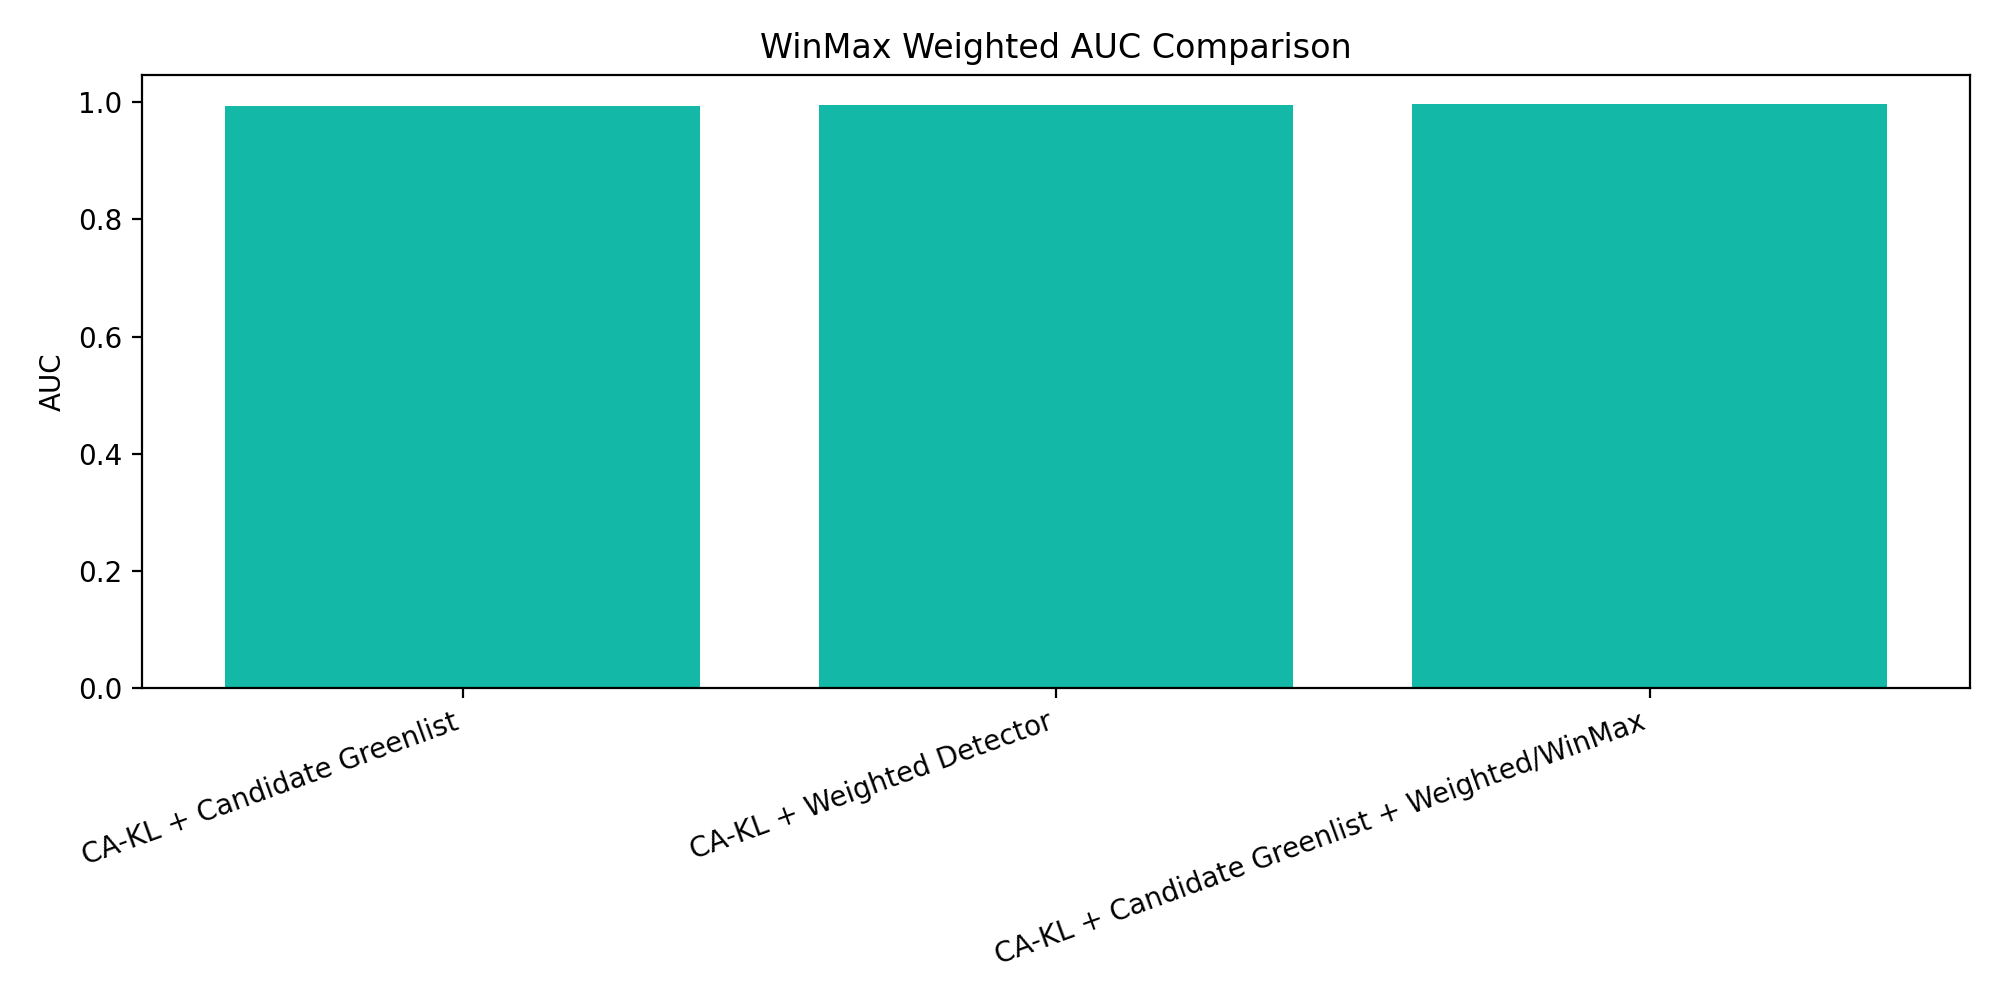
\includegraphics[width=0.86\textwidth]{cakl_weighted_auc.png}
    \caption{选定 gate 0.10/0.95 下 CA-KL 系列的 weighted AUC 对比}
    \label{fig:weighted-auc}
\end{figure}

\begin{figure}[H]
    \centering
    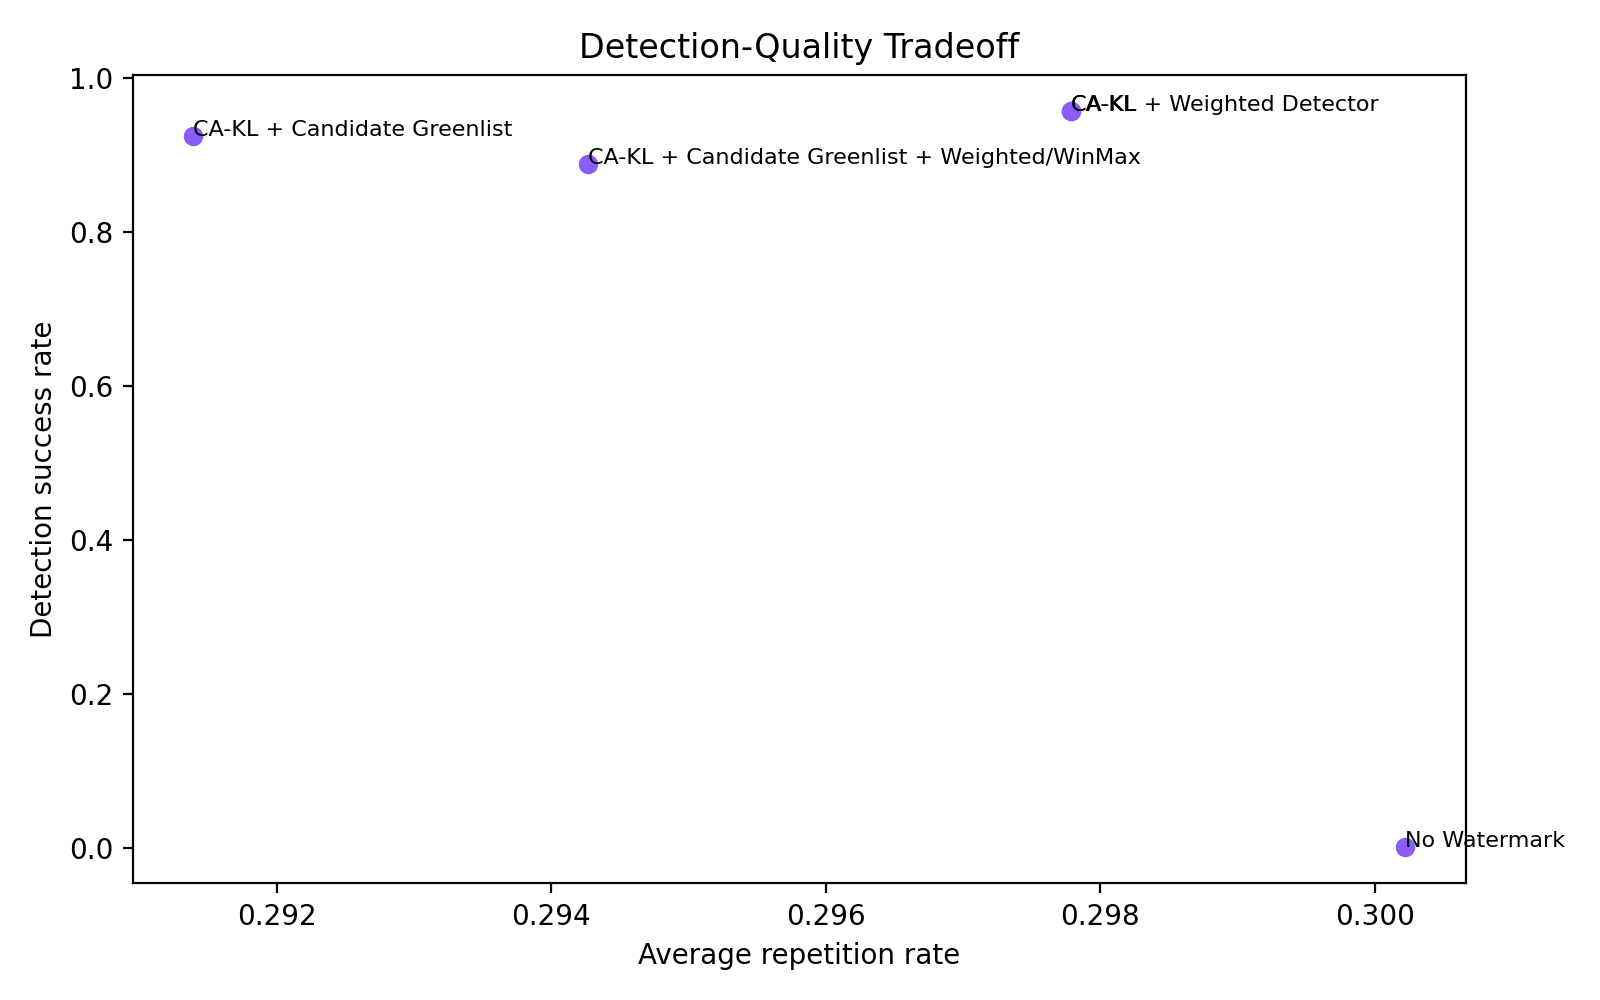
\includegraphics[width=0.86\textwidth]{cakl_tradeoff.png}
    \caption{选定 gate 0.10/0.95 下 CA-KL 系列的检测率与重复率折中}
    \label{fig:tradeoff}
\end{figure}

\subsection{KL 预算与自适应强度分析}

KL 预算 $\varepsilon$ 直接控制每一步允许的分布扰动。小规模网格实验比较了 $\varepsilon=0.30,0.35,0.40,0.50$；当 $\varepsilon$ 过小时，平均 \texttt{delta} 较低，水印信号不足。$\varepsilon=0.50$ 能使 \method{} 的平均 \texttt{delta} 接近 2.5，检测率进入稳定区间，因此正式实验采用该参数。在 500 条样本上，\method{} 的平均 \texttt{delta} 为 2.5108，CA-KL + Candidate Greenlist 为 2.4861，而加入 gate 后的 \fullmethod{} 降到 1.6893。

\begin{figure}[H]
    \centering
    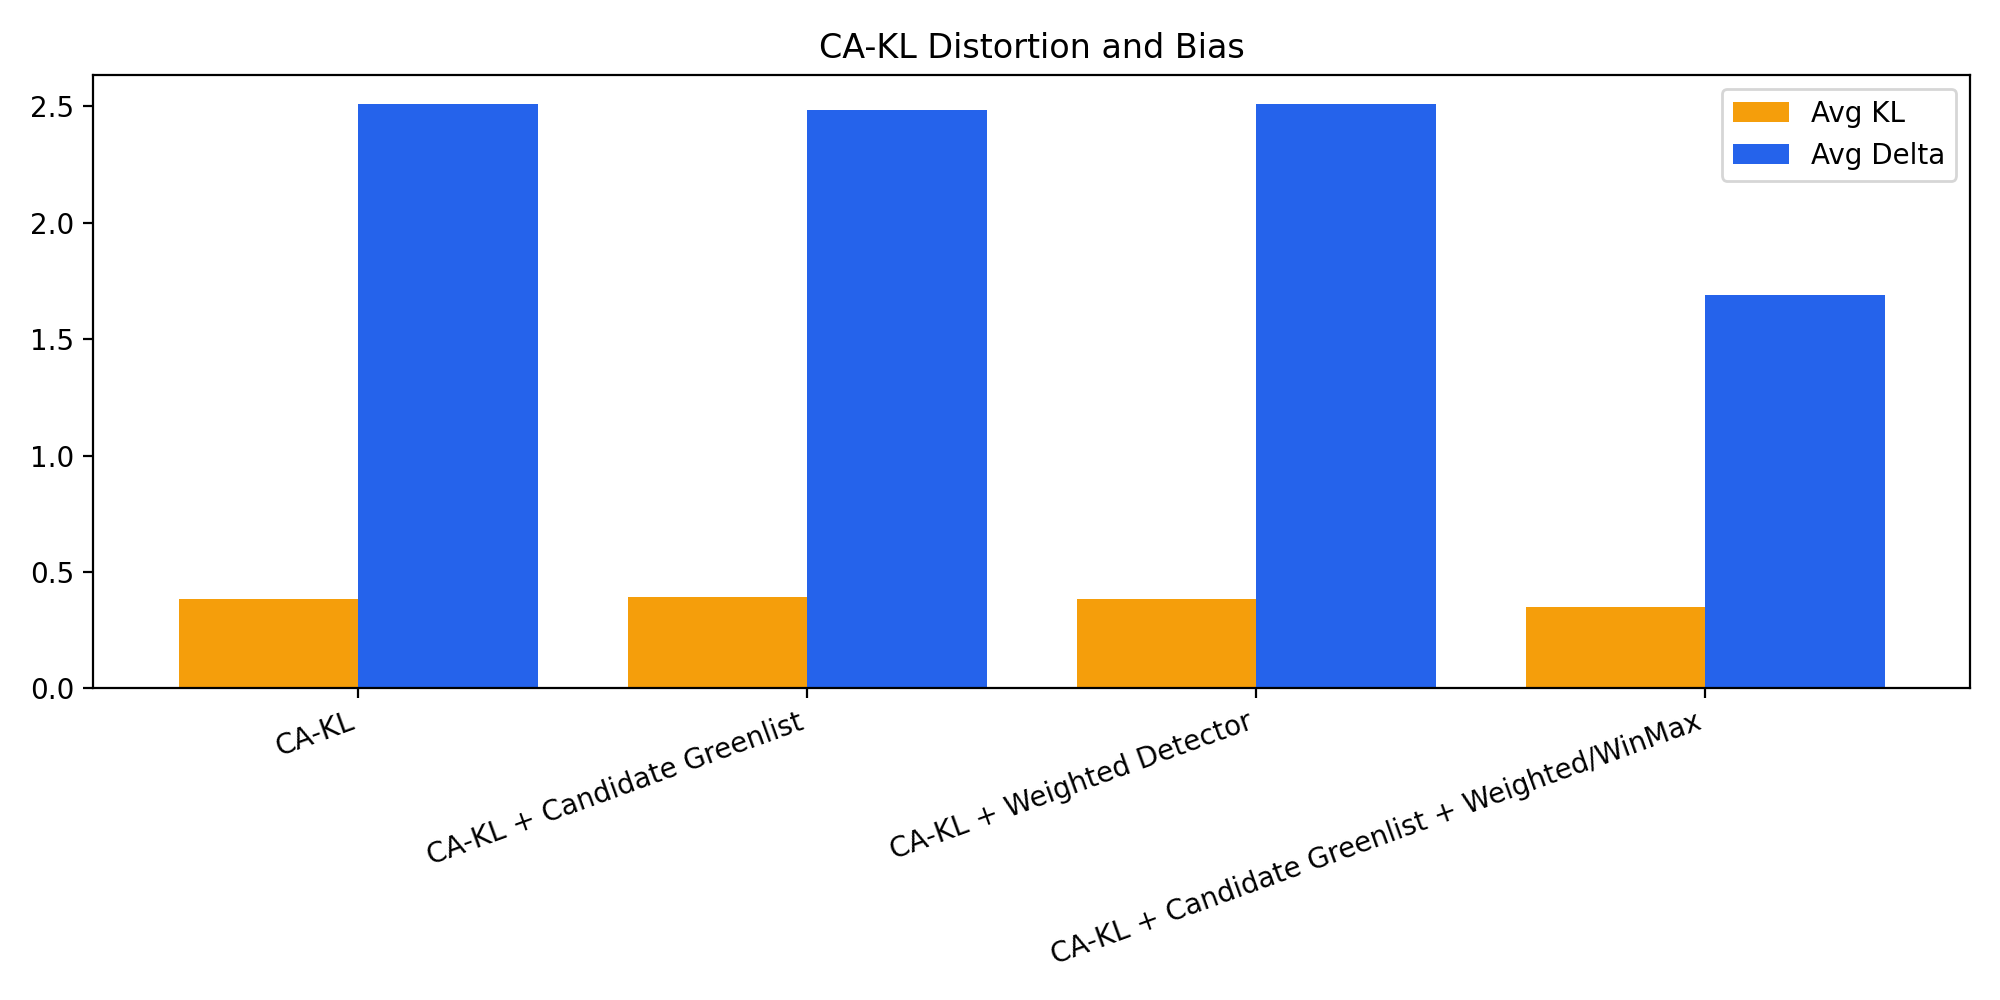
\includegraphics[width=0.86\textwidth]{cakl_kl_delta.png}
    \caption{CA-KL 方法中的平均 KL 与平均自适应 delta}
    \label{fig:kl-delta}
\end{figure}

KL 预算和 confidence gate 共同决定最终扰动强度。预算越大，可用偏置上界越高；gate 越严格，实际施加偏置的位置越少。\fullmethod{} 在 gate 0.10/0.95 下的平均 \texttt{delta} 约为 1.69，低于 \method{} 的 2.51，但在 weighted detector 下仍保持较高检测分数。这说明 KL 预算负责约束单步分布扰动，confidence gate 负责筛选适合嵌入的位置，两者共同构成完整的自适应水印强度控制机制。

\section{总结}

本报告完成了 KGW 文本水印方法的复现，并在固定 \texttt{delta} 的基础上实现了两类自适应水印机制。Adaptive Delta 通过 next-token 分布熵调整偏置强度，提供了直观的可嵌入性建模；\method{} 则进一步使用 KL 散度预算约束每一步分布扰动，使水印强度具有明确的统计解释。\fullmethod{} 在此基础上加入 candidate-aware greenlist 和 confidence gate，把水印嵌入集中到候选空间内更合适的位置。

500 条 OPT-2.7B fp32 实验表明，\method{} 在普通 KGW 检测器下的检出率为 95.60\%，高于 \texttt{Fixed Delta 2.0} 的 92.80\% 和 Adaptive Delta 的 88.60\%，说明 KL 约束水印能够形成稳定检测信号。\fullmethod{} 在 gate 0.10/0.95 下的普通 KGW 检出率为 88.80\%，PPL 为 5.6073，平均 \texttt{delta} 为 1.6893；与平均强度接近的 \texttt{Fixed Delta 1.7} 相比，普通 KGW 检出率从 82.00\% 提升到 88.80\%。在模型辅助 weighted/WinMax detector 下，\fullmethod{} 的 weighted z-score AUC 达到 0.9992，TPR@1\%FPR 达到 99.60\%，表明自适应生成留下的水印证据可以被匹配检测器稳定捕捉。

综上，本文的主要贡献包括：第一，复现并系统比较固定 \texttt{delta}、Adaptive Delta、\method{} 和 \fullmethod{}；第二，提出 KL 预算下的动态水印强度控制机制，使每一步 \texttt{delta} 由分布扰动约束决定；第三，实现 candidate-aware greenlist、confidence gate 与模型辅助 weighted/WinMax detector，使生成端自适应嵌入和检测端统计量形成对应关系。实验结果说明，该方法能够在可解释扰动约束下保持较强检测信号，并为后续研究自适应文本水印提供了可复现实验框架。


\clearpage
\bibliographystyle{ieeetr}
\bibliography{reference}

\appendix
\section{核心代码片段}

下面列出 \method{} 中 KL 约束求解的核心逻辑。完整代码位于 \codepath{course_project/processors/cakl_watermark_processor.py}。

\begin{lstlisting}[language=Python]
def _kl_for_delta(self, delta: float, p_green_mass: float) -> float:
    if delta <= 0.0 or p_green_mass <= 0.0:
        return 0.0
    normalizer = 1.0 + (exp(delta) - 1.0) * p_green_mass
    q_green_mass = exp(delta) * p_green_mass / normalizer
    return delta * q_green_mass - log(normalizer)

def _solve_delta(self, p_green_mass: float) -> tuple[float, float]:
    if self.kl_epsilon <= 0.0 or self.delta_max <= 0.0:
        return 0.0, 0.0
    if self._kl_for_delta(self.delta_max, p_green_mass) <= self.kl_epsilon:
        return self.delta_max, self._kl_for_delta(self.delta_max, p_green_mass)
    lo, hi = 0.0, self.delta_max
    for _ in range(self.binary_search_steps):
        mid = (lo + hi) / 2.0
        if self._kl_for_delta(mid, p_green_mass) <= self.kl_epsilon:
            lo = mid
        else:
            hi = mid
    return lo, self._kl_for_delta(lo, p_green_mass)
\end{lstlisting}

\end{document}
